\chapter{Marco Conceptual}

\section{Sistema de información} 	
\setlength{\parskip}{5mm}
Los SI son conjuntos organizados de elementos dirigidos a recoger, procesar, almacenar y distribuir información de manera que pueda ser utilizada por las personas adecuadas dentro de las empresas, de modo que desempeñen sus actividades de manera eficaz y eficiente” (Colomina, 1998)

Desde el punto de vista empresarial, los sistemas de información tienen como propósito perfeccionar las actividades llevadas a cabo en una organización, y así alcanzar ventajas competitivas.

\setlength{\parskip}{0mm}


\section{Tipos de sistemas de información} 	

\subsection{Sistema de procesamiento de transacciones (TPS)}
\setlength{\parskip}{5mm}
Cuando un sistema recopila, almacena y altera la información creada a partir de transacciones llevadas a cabo dentro de una organización se denomina sistema de procesamiento de transacciones. Tiene como finalidad procesar las transacciones diarias de una empresa, acumulando toda la información recibida en una base de datos para su posterior consulta.

\setlength{\parskip}{0mm}

\subsection{Sistema de información gerencial (MIS)}
\setlength{\parskip}{5mm}
Un sistema de información gerencial es aquel utilizado por la empresa para solventar inconvenientes en la misma. Es decir, el objetivo del mismo es la suministración de información para la resolución de problemas a través de la interacción entre tecnologías y personas.

Los datos aportados por el sistema deben disponer de cuatro cualidades elementales: calidad, oportunidad, cantidad y relevancia.

\setlength{\parskip}{0mm}

\subsection{Sistema de apoyo a la toma de decisiones (DSS)}
\setlength{\parskip}{5mm}

Este sistema se basa en el estudio y la comparación entre un conjunto de variables con el objeto de contribuir a la toma de decisiones dentro de una empresa. El apoyo dado por el sistema involucra la estimación, valoración y balance entre alternativas. Al igual que el sistema de información gerencial, esta tecnología interacciona con personas en el filtrado de información que permite optar por la decisión mas acertada.


% Las principales características de estos son:

%     Suelen introducirse después de haber implantado los Sistemas Transaccionales más relevantes de la empresa, ya que estos últimos constituyen su plataforma de información.

%     La información que generan sirve de apoyo a los mandos intermedios y a la alta administración en el proceso de toma de decisiones.

% Suelen ser intensivos en cálculos y escasos en entradas y salidas de información. Así, por ejemplo, un modelo de planeación financiera requiere poca información de entrada, genera poca información como resultado, pero puede realizar muchos cálculos durante su proceso.

%     No suelen ahorrar mano de obra. Debido a ello, la justificación económica para el desarrollo de estos sistemas es difícil, ya que no se conocen los ingresos del proyecto de inversión.

%     Suelen ser Sistemas de Información interactivos y amigables, con altos estándares de diseño gráfico y visual, ya que están dirigidos al usuario final.

%     Apoyan la toma de decisiones que, por su misma naturaleza son repetitivos y de decisiones no estructuradas que no suelen repetirse. Por ejemplo, un Sistema de Compra de Materiales que indique cuándo debe hacerse un pedido al proveedor o un Sistema de Simulación de Negocios que apoye la decisión de introducir un nuevo producto al mercado.

%     Estos sistemas pueden ser desarrollados directamente por el usuario final sin la participación operativa de los analistas y programadores del área de informática.

% Este tipo de sistemas puede incluir la programación de la producción, compra de materiales, flujo de fondos, proyecciones financieras, modelos de simulación de negocios, modelos de inventarios, entre otros.


% https://richardunefa.wordpress.com/principios-de-sistemas-de-informacion/

\setlength{\parskip}{0mm}

\subsection{Sistema de información ejecutiva (EIS)}
\setlength{\parskip}{5mm}
 Esta tecnología es utilizada por los gerentes de una empresa, ya que permite acceder a la información interna y externa de la misma, disponiendo de los datos que puedan llegar a afectar su buen rendimiento.
De esta manera, el ejecutivo podrá conocer el estado de todos los indicadores, incluso aquellos que no cumplan con las expectativas y a partir de esto, tomar las medidas que considere adecuadas.
\setlength{\parskip}{0mm}


% http://www.tiposde.org/informatica/89-tipos-de-sistemas-de-informacion/
% http://www.monografias.com/trabajos7/sisinf/sisinf2.shtml


\section{Base de Datos} 	
\setlength{\parskip}{5mm}
``Una base de datos (cuya abreviatura es BD) es una entidad en la cual se pueden almacenar datos de manera estructurada, con la menor redundancia posible.''(\cite{bdbib})
Diferentes programas y diferentes usuarios deben poder utilizar estos datos. Por lo tanto, el concepto de base de datos generalmente está relacionado con el de red ya que se debe poder compartir esta información. De allí el término base. Sistema de información es el término general utilizado para la estructura global que incluye todos los mecanismos para compartir datos que se han instalado. %(\citet{bdbib}, 2016) 


\setlength{\parskip}{0mm}



\subsection{Sistema Manejador de Base de Datos}
\setlength{\parskip}{5mm}

``Un sistema manejador de bases de datos (SGBD, por sus siglas en inglés) o DataBase Management System (DBMS) es una colección de software muy específico, cuya función es servir de interfaz entre la base de datos, el usuario y las distintas aplicaciones utilizadas.'' (\citet{smdbbib})

Como su propio nombre indica, el objetivo de los sistemas manejadores de base de datos es precisamente el de manejar un conjunto de datos para convertirlos en información relevante para la organización, ya sea a nivel operativo o estratégico.
 
Lo hace mediante una serie de rutinas de software para permitir su uso de una manera segura, sencilla y ordenada. Se trata, en suma, de un conjunto de programas que realizan tareas de forma interrelacionada para facilitar la construcción y manipulación de bases de datos, adoptando la forma de interfaz entre éstas, las aplicaciones y los mismos usuarios. 

El SMDB puede dividirse en tres subsistemas:
\setlength{\parskip}{0mm}
\begin{itemize}

    \item El sistema de administración de archivos: para almacenar información en un medio físico
    
    \item El DBMS interno: para ubicar la información en orden
    
    \item El DBMS externo: representa la interfaz del usuario

\end{itemize}



\setlength{\parskip}{5mm}
A continuación se presentarán algunos ejemplos de SMBD.
\setlength{\parskip}{0mm}

\subsection {PostgresSQL}
\setlength{\parskip}{5mm}
\cite{postgresbib} afirma: ``PostgreSQL es un sistema de gestión de bases de datos objeto-relacional, distribuido bajo licencia BSD y con su código fuente disponible libremente. Es el sistema de gestión de bases de datos de código abierto más potente del mercado.''

PostgreSQL utiliza un modelo cliente/servidor y usa multi-procesos en vez de multi-hilos para garantizar la estabilidad del sistema. Un fallo en uno de los procesos no afectará el resto y el sistema continuará funcionando.

Sus características técnicas la hacen una de las bases de datos más potentes y robustas del mercado. Su desarrollo comenzó hace más de 16 años, y durante este tiempo, estabilidad, potencia, robustez, facilidad de administración e implementación de estándares han sido las características que más se han tenido en cuenta durante su desarrollo.

PostgreSQL funciona muy bien con grandes cantidades de datos y una alta concurrencia de usuarios accediendo a la vez a el sistema.
\setlength{\parskip}{0mm}


%\url{http://www.postgresql.org.es/sobre_postgresql}
\newpage
\subsection{MySQL}
\setlength{\parskip}{5mm}
MySQL es un sistema de administración de bases de datos (Database Management System, DBMS) para bases de datos relacionales. Así, MySQL no es más que una aplicación que permite gestionar archivos llamados de bases de datos.

\citet{mysqlbib} mencionan: ``MySQL, como base de datos relacional, utiliza múltiples tablas para almacenar y organizar la información. MySQL fue escrito en C y C++ y destaca por su gran adaptación a diferentes entornos de desarrollo, permitiendo su interacción con los lenguajes de programación más utilizados como PHP, Perl y Java y su integración en distintos sistemas operativos.''

También es muy destacable, la condición de open source de MySQL, que hace que su utilización sea gratuita e incluso se pueda modificar con total libertad, pudiendo descargar su código fuente. Esto ha favorecido muy positivamente en su desarrollo y continuas actualizaciones, para hacer de MySQL una de las herramientas más utilizadas por los programadores orientados a Internet.
\setlength{\parskip}{0mm}
%(, 2005)
%http://www.esepestudio.com/noticias/que-es-mysql

\subsection{Oracle}
\setlength{\parskip}{5mm}
``Oracle la Primera Base de Datos Diseñada para Grid Computing, es un sistema de gestión de base de datos relacional fabricado por Oracle Corporation. Oracle es básicamente un herramienta cliente/servidor para la gestión de base de datos la gran potencia que tiene y su elevado precio hace que solo se vea en empresas muy grandes y multinacionales, por norma general. Oracle Corporation :es una de las mayores compañías de software del mundo. Sus productos van desde bases de datos (Oracle) hasta sistemas de gestión. Cuenta además, con herramientas propias de desarrollo para realizar potentes aplicaciones, como Oracle Designer.""(\citet{oraclebib})

Desarrollado sobre Oracle Database, Oracle Content Database ha sido diseñada para que las organizaciones puedan controlar y gestionar grandes volúmenes de contenidos no estructurados en un único repositorio con el objetivo de reducir los costes y los riesgos asociados a la pérdida de información.
\setlength{\parskip}{0mm}


\newpage
\subsection{Cuadro Comparativo SMBD}
\begin{table}[H]	
\begin{center}
\begin{tabular}{ | m{3cm} | m{4.5cm}| m{4.5cm}| } 
 \hline
 SMDB & Ventajas & Desventajas \\
 \hline
 PostgresSQL 
 &
 %ventajas
 - Multiplataforma.
 \newline
 - Diseñado para ambientes de alto volumen.
 \newline
 - Herramientas gráficas de diseño y administración.
 \newline
 - Tiene mejor soporte que los proveedores comerciales.
 \newline
 - Licencia abierta.
 &
 %desvantajas \\
-La sintaxis de algunos de sus comandos o sentencias no es nada intuitiva.
\newline
-Es más lento en inserciones y actualizaciones, ya que cuenta con cabeceras de intersección que no tienen otros SMBD.
\newline
-El soporte es en línea.
\\
  \hline
 MySQL
 &
 %ventajas
 - Tiene una mayor velocidad al realizar operaciones.
  \newline
 - Baja probabilidad de corromper datos.
  \newline
 - Característica única puede agrupar transacciones.
  \newline
 - Permite la gestión de diferentes usuarios y permisos.
  \newline
 - Es Licencia abierta.
 &
 %desvantajas
 -Un gran porcentaje de las utilidades de MySQL no están documentadas.
 \newline
 -Poco intuitivo.
 \\
 \hline
 Oracle
 &
 %ventajas
 - Es considerado como uno de los sistemas gestores de bases de datos más completo.
  \newline
 - Permite el uso de particiones.
  \newline
 - Consultas en paralelo.
  \newline
 - Las herramientas de configuración de Oracle son tal vez las mejores en el mercado.
 &
 %desvantajas
 
 - Un Oracle mal configurado puede ser desesperadamente lento.
  \newline
  - Es privativo, costos no muy asequibles.
 \\
 \hline
 \end{tabular}
\caption{Tabla comparativa de los Sistemas Manejadores de Base de Datos}
\label{Tabla:3}
\end{center}
\end{table}	

\newpage
%https://iessanvicente.com/colaboraciones/oracle.pdf




\section{Tecnologías de desarrollo web}

\subsection{HTML}

\setlength{\parskip}{5mm}

HTML, sigla en inglés de HyperText Markup Language (lenguaje de marcas de hipertexto), hace referencia al lenguaje de marcado para la elaboración de páginas web. Es un estándar que sirve de referencia del software que conecta con la elaboración de páginas web en sus diferentes versiones, define una estructura básica y un código (denominado código HTML) para la definición de contenido de una página web, como texto, imágenes, vídeos, juegos, entre otros. (\citet{htmlbib})

Los documentos HTML son descritos por las etiquetas HTML, cada etiqueta HTML describe diferentes contenidos de documentos.

\setlength{\parskip}{0mm}

\subsection{CSS}
\setlength{\parskip}{5mm}
Hoja de estilo en cascada o CSS (siglas en inglés de cascading style sheets) es un lenguaje usado para definir y crear la presentación de un documento estructurado escrito en HTML o XML.(\cite{cssbib}) 

La idea que se encuentra detrás del desarrollo de CSS es separar la estructura de un documento de su presentación. Es usado para definir los estilos de nuestra pagina web, incluyendo diseño, layouts y una variedad de vistas en los diferentes dispositivos y sus tamaños de pagina.
\setlength{\parskip}{0mm}

\subsection{JavaScript}
\setlength{\parskip}{5mm}
Javascript es un lenguaje de programación interpretado, dialecto del estándar ECMAScript. Se define como orientado a objetos, basado en prototipos, imperativo, débilmente tipeado y dinámico.(\cite{javascripbib})

Se utiliza principalmente en su forma del lado del cliente, implementado como parte de un navegador web permitiendo mejoras en la interfaz de usuario y páginas web dinámicas aunque existe una forma de JavaScript del lado del servidor (Server-side JavaScript o SSJS). Su uso en aplicaciones externas a la web, por ejemplo en documentos PDF, aplicaciones de escritorio es también significativo.

Tradicionalmente se venía utilizando en páginas web HTML para realizar operaciones y únicamente en el marco de la aplicación cliente, sin acceso a funciones del servidor. Actualmente es ampliamente utilizado para enviar y recibir información del servidor junto con ayuda de otras tecnologías como AJAX. JavaScript se interpreta en el agente de usuario al mismo tiempo que las sentencias van descargándose junto con el código HTML.
\setlength{\parskip}{0mm}


\subsection{JQuery}
\setlength{\parskip}{5mm}
\cite{jquerybib} sostiene que: jQuery es una biblioteca de JavaScript, creada inicialmente por John Resig, que permite simplificar la manera de interactuar con los documentos HTML, manipular el árbol DOM, manejar eventos, desarrollar animaciones y agregar interacción con la técnica AJAX a páginas web. Fue presentada el 14 de enero de 2006 en el BarCamp NYC. jQuery es la biblioteca de JavaScript más utilizada. 

jQuery es software libre y de código abierto, posee un doble licenciamiento bajo la Licencia MIT y la Licencia Pública General de GNU v2, permitiendo su uso en proyectos libres y privados. jQuery, al igual que otras bibliotecas, ofrece una serie de funcionalidades basadas en JavaScript que de otra manera requerirían de mucho más código, es decir, con las funciones propias de esta biblioteca se logran grandes resultados en menos tiempo y espacio.
\setlength{\parskip}{0mm}
%(\citet{jquerybib}, 2009)
%http://www.desarrolloweb.com/articulos/introduccion-jquery.html

\subsection{JQueryUI}
\setlength{\parskip}{5mm}
\citet{jqueryuibib} establece que: jQuery UI es un complemento que permite implementar componentes diversos para generar interfaces de usuario en páginas web, además de otras funcionalidades básicas para crear aplicaciones web enriquecidas. Como su propio nombre indica, está basado en el popular framework Javascript y podemos encontrar links, explicaciones, así como demos y descargas a partir del sitio web oficial de jQuery.

Es una biblioteca de componentes y cada componente o módulo se desarrolla de acuerdo a la filosofía de jQuery (find something, manipulate it: encuentra algo, manipúlalo).
\setlength{\parskip}{0mm}
%(\citet{jqueryuibib}, 2013)
%http://www.desarrolloweb.com/manuales/manual-jqueryui.html

\subsection{Boopstrap}
\setlength{\parskip}{5mm}
Bootstrap o twitter-bootstrap es un framework creado originalmente por dos desarrolladores/diseñadores de twitter para acelerar el diseño de nuevas aplicaciones web.

``El framework proporciona clases css y código javascript para definir el layout de la página, crear componentes que respondan a eventos y estilizar los elementos html más habituales.''(\cite{bootstrap})

La mayor ventaja es que podemos crear interfaces que se adapten a los distintos navegadores (responsive design) apoyándonos en un framework potente con numerosos componentes webs que nos ahorrarán mucho esfuerzo y tiempo. 

Podemos decir que los principios en los que se basa son:
\setlength{\parskip}{0mm}
\begin{itemize}

	\item Responsive Design: consiste en que la página trata de “hacer lo correcto” al ser visualizada independientemente del dispositivo y tamaño de la pantalla
	
	\item Mobile first: Al contrario que en la versión 2, en la 3, el diseño responsivo es la opción por defecto al trabajar con bootstrap

	\item Cross Browser: Trata de ser compatible con la mayoría de navegadores.
	
	\item Integración con jQuery: Está muy integrado con jquery para el que define nuevos plugins

	\item Buenas prácticas: Trata de emplear algunas de las prácticas más extendidas en cuanto a usabilidad, uso de css3/html5, organización del código
	
	
\end{itemize}

\subsection{Django}
\setlength{\parskip}{5mm}
\citet{djangobib} estipula que: Django es un framework de desarrollo web de código abierto, escrito en Python, que respeta el patrón de diseño conocido como: Modelo–vista–controlador

La meta fundamental de Django es facilitar la creación de sitios web complejos. Django pone énfasis en el re-uso, la conectividad y extensibilidad de componentes, el desarrollo rápido y el principio No te repitas (DRY, del inglés Don't Repeat Yourself). Python es usado en todas las partes del framework, incluso en configuraciones, archivos, y en los modelos de datos.(\citet{djangobib})

Proporciona una serie de características que facilitan el desarrollo rápido de páginas orientadas a contenidos

Django fue desarrollado por Adrian Holovaty, Simon Willison, Jacob Kaplan-Moss y Wilson Miner mientras trabajaban en World Online, y originalmente se utilizó para administrar tres sitios web de noticias.

Los orígenes de Django en la administración de páginas de noticias son evidentes en su diseño, ya que proporciona una serie de características que facilitan el desarrollo rápido de páginas orientadas a contenidos. Por ejemplo, en lugar de requerir que los desarrolladores escriban controladores y vistas para las áreas de administración de la página, Django proporciona una aplicación incorporada para administrar los contenidos, que puede incluirse como parte de cualquier página hecha con Django y que puede administrar varias páginas hechas con Django a partir de una misma instalación; la aplicación administrativa permite la creación, actualización y eliminación de objetos de contenido, llevando un registro de todas las acciones realizadas sobre cada uno, y proporciona una interfaz para administrar los usuarios y los grupos de usuarios (incluyendo una asignación detallada de permisos).

La distribución principal de Django también aglutina aplicaciones que proporcionan un sistema de comentarios, herramientas para sindicar contenido via RSS y/o Atom, "páginas planas" que permiten gestionar páginas de contenido sin necesidad de escribir controladores o vistas para esas páginas, y un sistema de redirección de URLs.

Otras características de Django son:
\setlength{\parskip}{0mm}
\begin{itemize}

	\item Un mapeador objeto-relacional.
	
	\item Aplicaciones modulares que pueden instalarse en cualquier página gestionada con Django.
	
	\item Una API de base de datos robusta.
	
	\item Un sistema incorporado de "vistas genéricas" que ahorra tener que escribir la lógica de ciertas tareas comunes.
	
	\item Un sistema extensible de plantillas basado en etiquetas, con herencia de plantillas.
	
	\item Un despachador de URLs basado en expresiones regulares.
	
	\item Un sistema "middleware" para desarrollar características adicionales; por ejemplo, la distribución principal de Django incluye componentes middleware que proporcionan cacheo, compresión de la salida, normalización de URLs, protección CSRF y soporte de sesiones.
	
	\item Soporte de internacionalización, incluyendo traducciones incorporadas de la interfaz de administración.
	
	\item Documentación incorporada accesible a través de la aplicación administrativa (incluyendo documentación generada automáticamente de los modelos y las bibliotecas de plantillas añadidas por las aplicaciones).

\end{itemize}




\subsection{CakePHP}
\setlength{\parskip}{5mm}
\citet{cakebib} sostiene que: CakePHP es un marco de desarrollo [framework] rápido para PHP, libre, de código abierto. Se trata de una estructura que sirve de base a los programadores para que éstos puedan crear aplicaciones Web. Nuestro principal objetivo es que puedas trabajar de forma estructurada y rápida, sin pérdida de flexibilidad.

Con CakePHP el desarrollo web ya no es monótono porque ofrecemos las herramientas para que empieces a escribir el código que realmente necesitas: la lógica específica de tu aplicación. Consigue una copia de CakePHP, empieza con lo verdaderamente importante y no re-inventes la rueda cada vez que te incorpores a un nuevo proyecto.

CakePHP tiene un equipo de desarrolladores y una comunidad activos, lo que añade valor al proyecto. Con CakePHP, además de no tener que re-inventar la rueda, el núcleo de tu aplicación se mejora constantemente y está bien probado.

Esta es una lista breve con las características de las que disfrutarás al utilizar CakePHP:
\setlength{\parskip}{0mm}
\begin{itemize}

	\item Comunidad activa y amistosa

    \item Licencia flexible
    
    \item Compatible con PHP4 y PHP5
    
    \item CRUD integrado para la interacción con la base de datos
    
    \item Soporte de aplicación [scaffolding]
    
    \item Generación de código
    
    \item Arquitectura Modelo Vista Controlador (MVC)
    
    \item Despachador de peticiones [dispatcher], con URLs y rutas personalizadas y limpias
    
    \item Validación integrada
    
    \item Plantillas rápidas y flexibles (sintaxis de PHP, con ayudantes[helpers])
    
    \item Ayudantes para AJAX, Javascript, formularios HTML y más
    
    \item Componentes de Email, Cookie, Seguridad, Sesión y Manejo de solicitudes
    
    \item Listas de control de acceso flexibles
    
    \item Limpieza de datos
    
    \item Caché flexible
    
    \item Localización
    
    \item Funciona en cualquier subdirectorio del sitio web, con poca o ninguna configuración de Apache

	
	
\end{itemize}

%\url{http://book.cakephp.org/1.3/es/The-Manual/Beginning-With-CakePHP/What-is-CakePHP-Why-Use-it.html}

\subsection{Ruby on Rails}
\setlength{\parskip}{5mm}
\citet{rubybib} establece que Ruby on Rails es un entorno de desarrollo web de código abierto que está optimizado para la satisfacción de los programadores y para la productividad sostenible. Te permite escribir un buen código evitando que te repitas y favoreciendo la convención antes que la configuración.

Un conjunto de librerías, automatismos y convenciones destinados a resolver los problemas más comunes a la hora de desarrollar una aplicación web, para que el programador pueda concentrarse en los aspectos únicos y diferenciales de su proyecto en lugar de los problemas recurrentes.

Rails fue creado en 2003 por David Heinemeier Hansson y desde entonces ha sido extendido por el Rails core team, más de 2.100 colaboradores y soportado por una extensa y activa comunidad. %(\citet{rubybib}, s.f)

\setlength{\parskip}{0mm}


%http://www.rubyonrails.org.es/

\subsection{JSON}
\setlength{\parskip}{5mm}
JSON (JavaScript Object Notation - Notación de Objetos de JavaScript) es un formato ligero de intercambio de datos.Leerlo y escribirlo es simple para humanos, mientras que para las máquinas es simple interpretarlo y generarlo. Está basado en un subconjunto del Lenguaje de Programación JavaScript, Standard ECMA-262 3rd Edition - Diciembre 1999. 

\citet{jsonbib} establece que JSON es un formato de texto que es completamente independiente del lenguaje pero utiliza convenciones que son ampliamente conocidos por los programadores de la familia de lenguajes C, incluyendo C, C++, C, Java, JavaScript, Perl, Python, y muchos otros. Estas propiedades hacen que JSON sea un lenguaje ideal para el intercambio de datos. %(\citet{jsonbib}, 2016)

JSON está constituido por dos estructuras:
 \setlength{\parskip}{0mm}
\begin{itemize}

	\item Una colección de pares de nombre/valor. En varios lenguajes esto es conocido como un objeto, registro, estructura, diccionario, tabla hash, lista de claves o un arreglo asociativo.
	
	\item Una lista ordenada de valores. En la mayoría de los lenguajes, esto se implementa como arreglos, vectores, listas o sequencias.

	
\end{itemize}

%http://www.json.org/json-es.html

\section{El Seguro}	
\setlength{\parskip}{5mm}
	``El seguro constituye la forma más perfecta y técnicamente eficaz para la cobertura de riesgos -transformando los individuales en colectivos- y transfiriéndolos a una organización -el asegurador- estructurada con la técnica y operativa adecuadas para garantizar su compensación, en caso de ocurrir el evento.'' \cite{seguroIbib}
\setlength{\parskip}{0mm}

\subsection{Contrato del seguro}
\setlength{\parskip}{5mm}

	El contrato de seguro, es aquel contrato mediante el cual una persona llamada asegurador se obliga, a cambio de una suma de dinero, conocida como prima, a indemnizar a otra llamada asegurado o a la persona que este designe, beneficiario, de un perjuicio o daño que pueda causar un suceso incierto. De tal manera que la suma objeto de indemnización, que fue pactada expresamente, sea pagada cuando ocurra el suceso o riesgo cubierto por el seguro. %(\citeauthor{contratobib}, \citeyear{contratobib})

\setlength{\parskip}{0mm}

% \subsubsection{Características}

% \begin{itemize}

% 	\item Es un acto de comercio.- Efectivamente el contrato de seguro constituye un contrato mercantil, regulado en el Código de Comercio y en otros aspectos supletoriamente por la legislación civil.

% 	\item Es un contrato solemne.- El contrato de seguro es solemne, ya que su perfeccionamiento se produce a partir del momento en que el asegurador suscribe la póliza, la firma del asegurador sirve para solemnizar el acuerdo previo de voluntades entre las partes contratantes, respecto a los elementos del seguro.

% 	\item Es un contrato bilateral.- En razón de que genera derechos y obligaciones para cada uno de los sujetos contratantes, GARRIGUES al respecto señala : "..el tomador de seguros se obliga a pagar la prima y el asegurador se obliga a una prestación pecuniaria: si bien esta prestación esta subordinada a un evento incierto, cual es la realización del siniestro".

% 	\item Es un contrato oneroso.- Es oneroso, porque significa para las partes un enriquecimiento y empobrecimiento correlativos. "Por cuanto al tomador del seguro se le impone la obligación de pagar la prima y al asegurador la asunción del riesgo de la que deriva la prestación del pago de la indemnización de la que queda liberado si no se ha pagado la prima antes del siniestro".

% 	\item Es un contrato aleatorio.- Es aleatorio porque tanto el asegurado como el asegurador están sometidos a una contingencia que puede representar para uno una utilidad y para el otro una pérdida. Tal contingencia consiste en la posibilidad de que se produzca el siniestro. Al respecto el profesor MONTOYA dice : " El carácter aleatorio del contrato no desaparece por el hecho de que las compañías aseguradoras dispongan de tablas estadísticas que les permite determinar el costo de los riesgos, en función de lo cual fijan el importe de las primas…. osea que si bien la actividad aseguradora en si es cada vez menos riesgosa en la medida del perfeccionamiento de los medios para determinar la frecuencia de los riesgos, el contrato sigue siendo aleatorio tratándose de cada contrato aislado y respecto del asegurado".

% 	\item Es un contrato de ejecución continuada.- Por cuanto los derechos de las partes o los deberes asignados a ellas se van desarrollando en forma continua, a partir de la celebración del contrato hasta su finalización por cualquier causa.

% 	\item Es un contrato de adhesión.- El seguro no es un contrato de libre discusión sino de adhesión. Las cláusulas son establecidas por el asegurador, no pudiendo el asegurado discutir su contenido, tan sólo puede aceptar o rechazar el contrato impuesto por el asegurador. Sólo podrá escoger las cláusulas adicionales ofrecidas por el asegurador, pero de ninguna manera podrá variar el contenido del contrato. Pero todo esto dependerá de la voluntad y de la flexibilidad que tenga cada empresa aseguradora.

% \end{itemize}




\subsection{Funciones del Seguro}
\setlength{\parskip}{5mm}

Existen diferentes funciones del seguro, entre ellas tenemos: 

\setlength{\parskip}{0mm}

\subsubsection{Funciones sociológicas del seguro}

\begin{itemize}
	\item Fomenta la  protección de todos los miembros de una familia o individuos.

	\item Estimula el sentido de responsabilidad frente a terceros, esencial para: abrir nuevas empresas, realizar nuevas inversiones, crear empleo, etc.

	\item Contribuye a la estabilidad social protegiendo contingencias derivadas de la vejez y enfermedades o 
	accidentes.

	\item Financia la prevención de riesgos mediante la reducción de primas. Así, aparte de la colaboración del seguro con otros sectores, en el aspecto individual se destaca el espíritu de previsión representado en el interés que muestra en la prevención de las consecuencias desfavorables de un evento.

\end{itemize}

\subsubsection{Funciones económicas del seguro}

\begin{itemize}
	\item Contribuye positivamente al desarrollo económico al eliminar riesgos y estabilizar los resupuestos económicos. Por esto, debe desarrollarse paralelamente al resto de las actividades económicas.

	\item El seguro es la única actividad económica que posee capacidad para generar ahorro y financiación de inversiones a largo plazo.% Existen otras instituciones financieras que aportan ahorro a largo plazo pero sólo el seguro lo hace con un esquema de ahorro y financiando un tipo de inversión (global y sistemática) sustancialmente distintos a los utilizados habitualmente por otros intermediarios.

\end{itemize}

\subsubsection{Funciones laborales del seguro}

\begin{itemize}

	\item El seguro participa en la consecución de empleo directo e indirecto. Se estima que en España casi 49.000 familias “viven del seguro” (empleados, agentes, corredores, peritos, liquidadores, abogados, actuarios y otros profesionales) y que el sector está financiando alrededor de 600.000 puestos de trabajo estable.

\end{itemize}

\subsection{Póliza de seguro}
\setlength{\parskip}{5mm}

	\cite{seguroIbib} menciona que la póliza es el documento principal del contrato de seguro, en donde constan los derechos y obligaciones de las partes, es un documento privado redactado en varios folios. Las condiciones generales están impresas, mientras las condiciones particulares están normalmente mecanografiadas. 

	% http://www.monografias.com/trabajos17/contrato-seguro/contrato-seguro.shtml#poliza#ixzz4M9kcfgxe

\setlength{\parskip}{0mm}


\subsection{Seguro de Vehículo}
\setlength{\parskip}{5mm}

\cite{seguroVehiculobib} establece que este tipo de seguro puede amparar tanto los daños propios como los daños causados a un tercero.

\begin{itemize}
	\item Cobertura Amplia: La aseguradora se compromete a  indemnizar al Asegurado, en exceso del deducible y hasta la suma asegurada indicada en el Cuadro Póliza, los daños materiales que sufra el Vehículo Asegurado en el período de vigencia de la Póliza, mientras el vehículo se encuentre en circulación, reposo o en transporte dentro de la República Bolivariana de Venezuela, que ocasione un Daño Parcial, General o No Recuperable, salvo aquellos casos expresamente excluidos en esta Póliza.

	\item Cobertura de indemnización por robo del vehículo:La aseguradora se compromete a indemnizar al Asegurado, en caso de quedar privado del uso del Vehículo Asegurado, como consecuencia directa de Robo o hurto, una cantidad diaria, desde el día en que se hayan cumplido los requisitos establecidos para notificar el reclamo, de acuerdo con lo establecido en las Condiciones Particulares de la póliza, hasta el día en que:

	a) La Empresa de Seguros haga efectiva la indemnización correspondiente, una vez transcurrido el plazo previsto en las Condiciones Generales de esta Póliza.

	b) Se haya recuperado el Vehículo Asegurado en caso robo o hurto. De ser el Asegurado quién recupere el Vehículo Asegurado, se compromete a comunicarlo por escrito a la Empresa de Seguros.

	Si el Vehículo Asegurado recuperado requiere reparación por daños sufridos a causa del robo o del hurto, la aseguradora continuará indemnizando la cantidad diaria hasta la fecha prevista para la entrega del mismo. En ningún caso, la indemnización superará el monto de los días o suma asegurada para esta cobertura indicado en el cuadro-recibo de la póliza.


	\item Cobertura de responsabilidad civil ( Daños a terceros): La Aseguradora se compromete a indemnizar la responsabilidad que pudiera corresponder al propietario o conductor del vehículo asegurado, por lesiones o daños a terceros dentro de Venezuela de acuerdo a la ley y reglamento de tránsito vigente hasta los límites indicados en el cuadro de la póliza.

	\item Asistencia legal y/o defensa penal: Al ocurrir un accidente de transito, esta póliza cubre los gastos por asistencia legal para liberar al conductor y vehículo en caso de ser detenidos, así como todos los gastos correspondientes a su defensa penal si es necesario. Está también cubre los casos de demanda en contra del asegurado.


	\item Cobertura de accidentes personales para ocupantes de vehículos: La Aseguradora se compromete a indemnizar al Asegurado o Beneficiario,  la suma asegurada indicada en el Cuadro Póliza, por las lesiones corporales que afecten la integridad física de los Ocupantes del Vehículo Asegurado, a consecuencia de un accidente amparado por la Póliza mientras se encuentren dentro, subiendo o bajando del Vehículo Asegurado y bajo las Condiciones estipuladas en las condiciones de la Póliza.


\end{itemize}

\setlength{\parskip}{0mm}

\subsection{El Perito}
\setlength{\parskip}{5mm}
	\citet{peritobib} estipula que el Perito es esencial en el engranaje de la compañía de seguros, pero para conocer la verdadera dimensión del trabajo del perito, analizamos sus funciones, que se resumen en tres grandes apartados:


\subsubsection{Aspectos técnicos}
\begin{itemize}

\item Valoración económica de los daños, elaborando la peritación y realizando la propuesta de indemnización a la compañía de seguros. Determinación del valor del bien asegurado, como, por ejemplo, el
valor venal, el valor de mercado, el valor de los restos y la propuesta del importe líquido de la indemnización, cuando se ha producido un siniestro total o una pérdida total.

\item Verificación de siniestros, para la realización de informes de uso interno para la compañía de seguros con la justificación técnica de la ocurrencia del siniestro. Pueden ser informes de rehúses parciales o totales, que pueden aportarse como prueba en un juicio. Los informes de reconstrucción de accidentes de tráfico, a partir de huellas y vestigios, mediante cálculos físicos y matemáticos, pueden ser también un apoyo para la determinación de la culpabilidad en el juicio. 

\item Revisión de riesgos, para la contratación de nuevas pólizas de vehículos de segunda mano con coberturas de daños propios, lunas, etc.

\item Control de calidad de la reparación, mediante la comprobación, en primer lugar, de que la reparación se ha llevado conforme a la peritación en todas y cada una de las partidas asignadas por el perito; a continuación, que la reparación se ha realizado con las debidas garantías técnicas, de calidad y seguridad para los ocupantes del vehículo. Por último, se analizarán los defectos en la reparación, para que sean subsanados por el taller.

\item Averías mecánicas: valoración y peritación de los daños mecánicos bajo la cobertura de pólizas de vehículos de renting y de pólizas de garantía de venta de vehículos usados.

\end{itemize}


\subsubsection{Aspectos administrativo-legales}
\begin{itemize}

\item Implicación en la tramitación del siniestro. El perito, en contacto con el tramitador y a través del sistema de gestión de la compañía de seguros, está al día de la tramitación de los siniestros, del tipo de pólizas que comercializa la compañía de seguros, de sus coberturas y exclusiones, de los convenios entre compañías y del conocimiento de la legislación de seguros.

\end{itemize}

\subsubsection{Aspecto negociador}
\begin{itemize}

\item El perito es la imagen de la compañía de seguros, ya que está en contacto con los asegurados, perjudicados, talleres, otras compañías, con lo que su actuación está sujeta a examen continuo, y su comportamiento, a ojos del asegurado, es, por extensión, el de la compañía de seguros. 

\item El perito debe aportar, en todo momento, argumentos y criterios técnicos en la negociación con el taller.

\item Ha de consensuar la peritación: debe llegar a acuerdos con el taller sobre todas y cada una de las partidas que componen una peritación.

\item Realiza asesoría legal: al estar en contacto con los asegurados y el taller, en muchas ocasiones, el perito se convierte en el asesor sobre los aspectos legales de los siniestros

\end{itemize}

\newpage

%(\citet{peritobib}, 2012)
\subsubsection{Inspección para asegurar un Vehículo}

\citet{peritoIVbib} establece que en el proceso de peritaje y/o inspección es muy importante realizar un registro fotográfico del vehículo antes de comenzar a realizar las operaciones de diagnóstico.

Esto se realiza primero, porque es necesario el registro para el informe generado a las aseguradoras y/o el cliente y segundo, para evitar futuras reclamaciones a la hora determinar el proceso de inspección.

También se debe señalar la importancia que cumple la inspección al interior del vehículo, como soporte o elemento de consulta durante la atención de un siniestro para comparar características del vehículo y elementos de contenido.

En resumen el perito esta encargado de realizar diferentes tipos de inspecciones, para un vehículo nuevo en la aseguradora, tales como:

\begin{itemize}

	\item Registro Fotográfico.

	\item Inspección Mecánica.

	\item Inspección Latonería.

	\item Inspección Pintura.

	\item Inspección Vidrios.

	\item Inspección Chasis.

	\item Inspección Interiores y guarnecidos.

\end{itemize}

%(\citet{peritoIVbib}, 2012)

\newpage

\subsubsection{Caso de Estudio}

\begin{figure}[H]
\begin{center}
	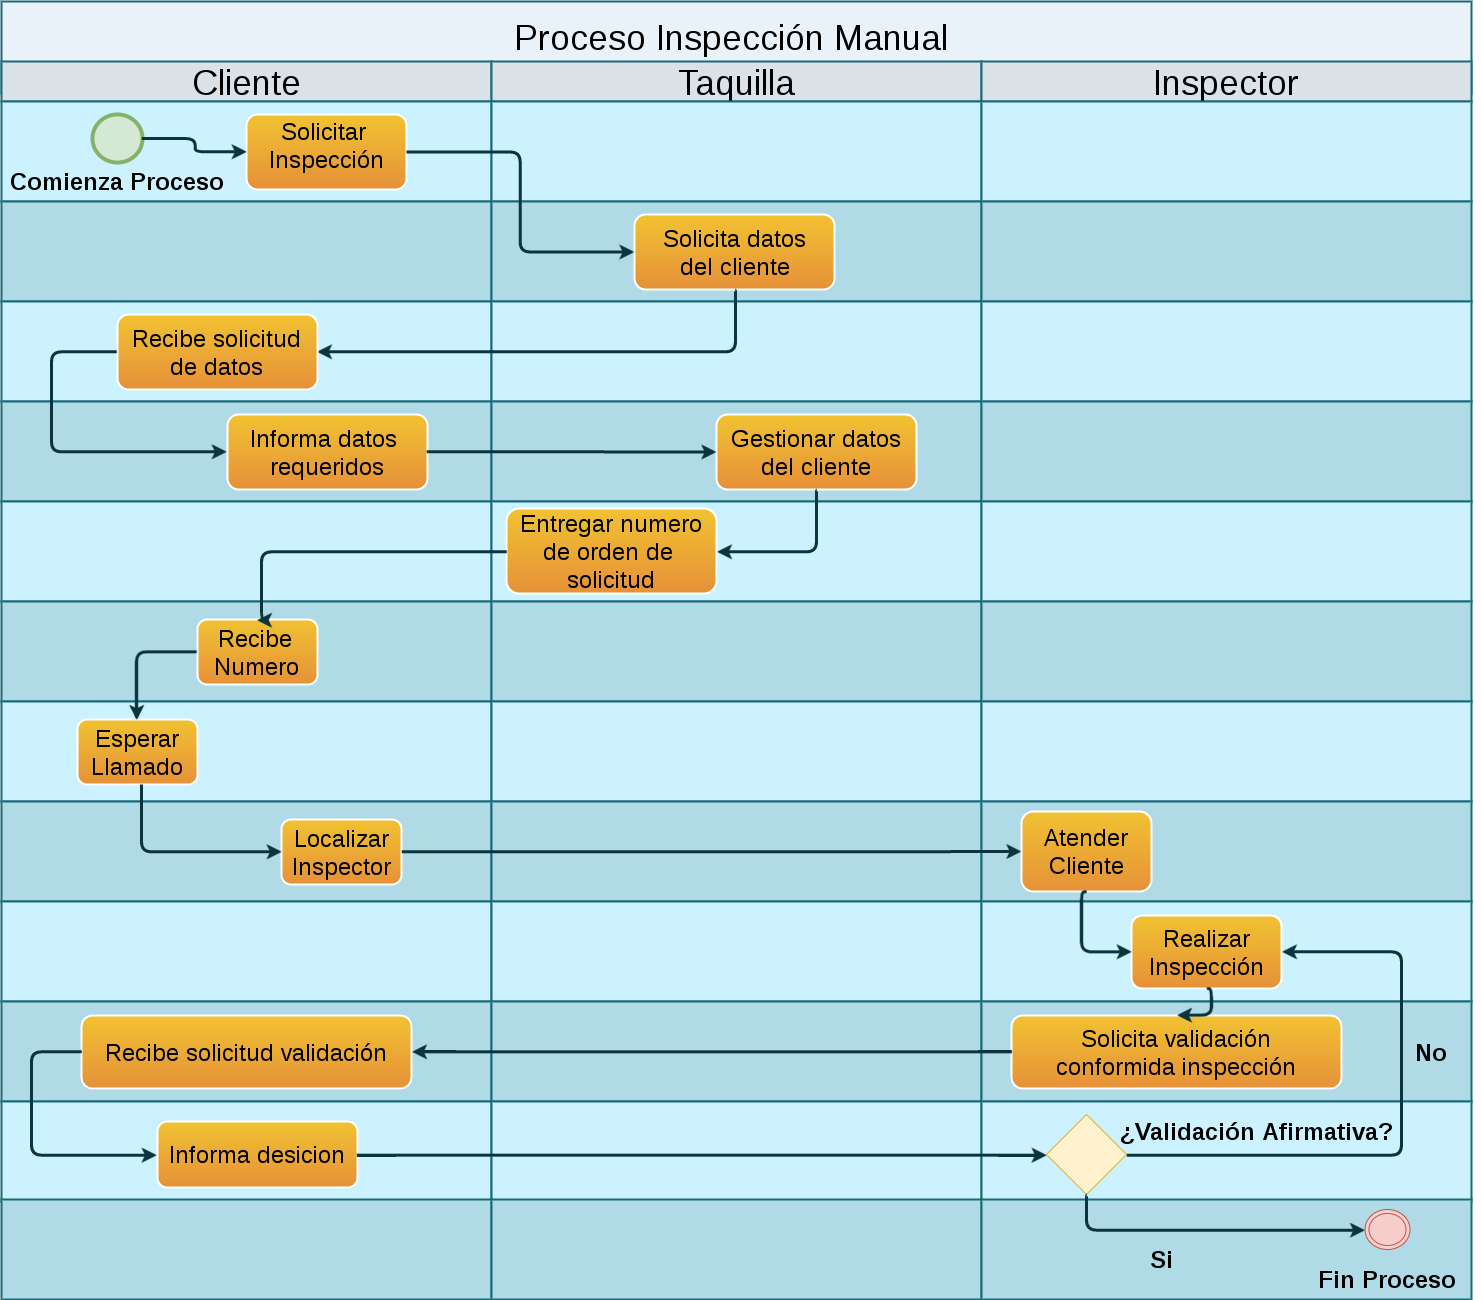
\includegraphics[width=\textwidth,height=15cm]{img/resumen_proceso.png}
\end{center}
\caption{Proceso Actual. (2016)}
\label{fig:proc_sin_sistema}
\end{figure}
\setlength{\parskip}{0mm}


\newpage

\subsubsection{Planilla de Suscripción}

\begin{figure}[H]
\begin{center}
	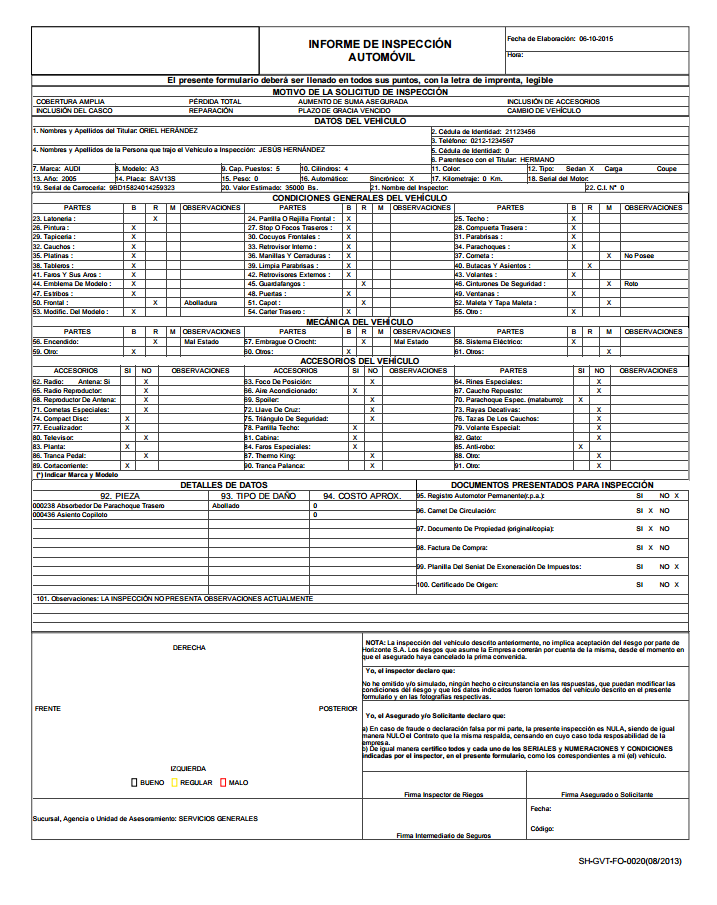
\includegraphics[width=\textwidth,height=18cm]{img/planilla_suscripcion.png}
\end{center}
\caption{Proceso de Suscripción. (2016)}
\label{fig:planilla_suscripcion}
\end{figure}
\setlength{\parskip}{0mm}